Per il progetto è stato sviluppato un plugin per Eclipse che si occupa di: \\*
\begin{itemize}
  \item text-highlight
  \item controllo degli errori
  \item compilazione
\end{itemize} 


\subsection{text-hilight}
Il plugin gestisce i file \emph{model} e \emph{layout} in modi differenti; i 
file, infatti, presentano caratteristiche e strutture diverse tra loro.
la classe che esegue la scansione del file e gestisce l'editor di \emph{model} è
la seguente:

\begin{lstlisting}[caption={ModelScanner}, style={java}]
public class ModelScanner extends RuleBasedScanner {
	//TODO controllare tutte le keyword
	private static String[] keywords= { "class","package", "public",
			"private","interface", "methods","extend", "relations", 
			"attributes"  };
	public ModelScanner(ColorManager manager) {
					manager.getColor(ColorConstants.DEFAULT)));
		ArrayList<IRule> rules= new ArrayList<IRule>();	
		Token tokencomment = new Token(new TextAttribute(
						manager.getColor(ColorConstants.COMMENT)));
		//Add rule for processing instructions
		rules.add( new SingleLineRule("//", "\n", tokencomment));
		rules.add( new SingleLineRule("#", "\n", tokencomment));
		rules.add( new MultiLineRule("/*", "*/", tokencomment));
		
		Token token= new Token(new TextAttribute(
				manager.getColor(ColorConstants.KEYWORD), 	//parola
				null, 	//sfondo
				SWT.BOLD));
		WordRule wordRule = new WordRule(new WordDetector());
		for (int i = 0; i < keywords.length; i++) {
			wordRule.addWord(keywords[i], token);
		}		
		rules.add(wordRule);
		
		token = new Token(new TextAttribute(
							manager.getColor(ColorConstants.BRACET)));
		RuleBrace braceRule = new RuleBrace(token);
		rules.add(braceRule);
		
		IRule[] r= new IRule[rules.size()];
		setRules(rules.toArray(r));
	}
}
\end{lstlisting}

la classe che esegue la scansione del file e gestisce l'editor di \emph{layout},
invece, è la seguente:

\begin{lstlisting}[caption={LayoutScanner}, style={java}]

prendere quella aggiornata


\end{lstlisting}

In entrambe le classi le parole chiave sono specificate nella stringa \emph{Keywords}, 
vengono definite le regole per i commenti, mentre per la gestione delle parentesi sono state 
definite delle regole comuni per entrambi i modelli.

\subsection{controllo degli errori}
il controllo degli errori viene eseguito ogni volta che il file viene salvato; a
livello di editor sono stati usati i marker laterali che indicano il tipo di
errore commesso (figura 2.1)

\begin{figure}[htp]
\begin{center}
  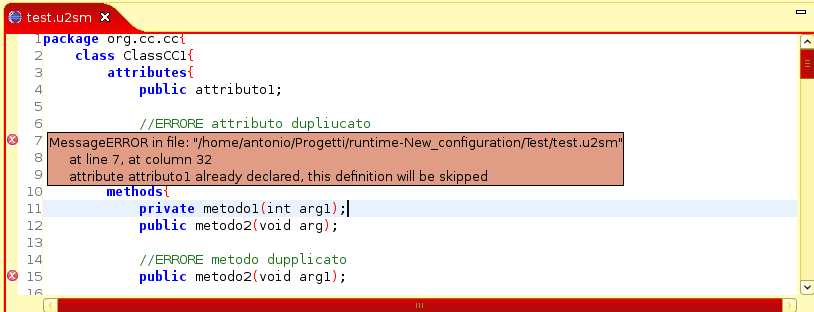
\includegraphics[width=0.9\textwidth]{img/errori_editor.png}
  \caption[labelInTOC]{Gestione degli errori}
\end{center}
\end{figure}